% Created by tikzDevice version 0.10.1 on 2017-11-29 19:14:32
% !TEX encoding = UTF-8 Unicode
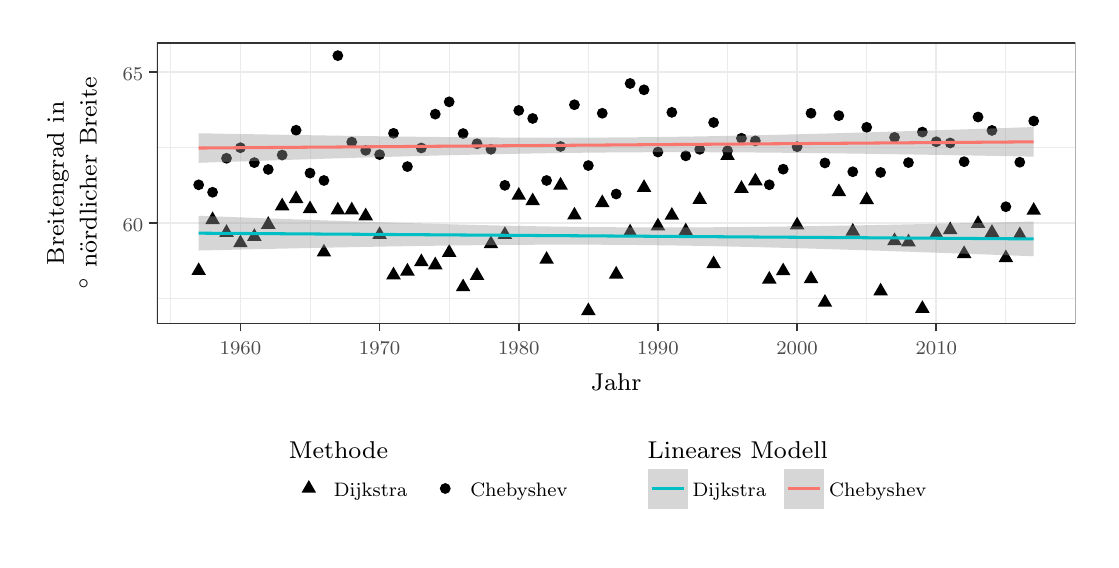
\begin{tikzpicture}[font=\footnotesize,x=1pt,y=1pt]
\definecolor{fillColor}{RGB}{255,255,255}
\path[use as bounding box,fill=fillColor,fill opacity=0.00] (0,0) rectangle (384.11,184.94);
\begin{scope}
\path[clip] (  0.00,  0.00) rectangle (384.11,184.94);
\definecolor{drawColor}{RGB}{255,255,255}
\definecolor{fillColor}{RGB}{255,255,255}

\path[draw=drawColor,line width= 0.6pt,line join=round,line cap=round,fill=fillColor] (  0.00,  0.00) rectangle (384.11,184.94);
\end{scope}
\begin{scope}
\path[clip] ( 46.70, 77.99) rectangle (378.61,179.44);
\definecolor{fillColor}{RGB}{255,255,255}

\path[fill=fillColor] ( 46.70, 77.99) rectangle (378.61,179.44);
\definecolor{drawColor}{gray}{0.92}

\path[draw=drawColor,line width= 0.3pt,line join=round] ( 46.70, 87.05) --
	(378.61, 87.05);

\path[draw=drawColor,line width= 0.3pt,line join=round] ( 46.70,141.70) --
	(378.61,141.70);

\path[draw=drawColor,line width= 0.3pt,line join=round] ( 51.73, 77.99) --
	( 51.73,179.44);

\path[draw=drawColor,line width= 0.3pt,line join=round] (102.02, 77.99) --
	(102.02,179.44);

\path[draw=drawColor,line width= 0.3pt,line join=round] (152.31, 77.99) --
	(152.31,179.44);

\path[draw=drawColor,line width= 0.3pt,line join=round] (202.60, 77.99) --
	(202.60,179.44);

\path[draw=drawColor,line width= 0.3pt,line join=round] (252.89, 77.99) --
	(252.89,179.44);

\path[draw=drawColor,line width= 0.3pt,line join=round] (303.18, 77.99) --
	(303.18,179.44);

\path[draw=drawColor,line width= 0.3pt,line join=round] (353.47, 77.99) --
	(353.47,179.44);

\path[draw=drawColor,line width= 0.3pt,line join=round] (378.61, 77.99) --
	(378.61,179.44);

\path[draw=drawColor,line width= 0.6pt,line join=round] ( 46.70,114.38) --
	(378.61,114.38);

\path[draw=drawColor,line width= 0.6pt,line join=round] ( 46.70,169.03) --
	(378.61,169.03);

\path[draw=drawColor,line width= 0.6pt,line join=round] ( 76.88, 77.99) --
	( 76.88,179.44);

\path[draw=drawColor,line width= 0.6pt,line join=round] (127.17, 77.99) --
	(127.17,179.44);

\path[draw=drawColor,line width= 0.6pt,line join=round] (177.46, 77.99) --
	(177.46,179.44);

\path[draw=drawColor,line width= 0.6pt,line join=round] (227.74, 77.99) --
	(227.74,179.44);

\path[draw=drawColor,line width= 0.6pt,line join=round] (278.03, 77.99) --
	(278.03,179.44);

\path[draw=drawColor,line width= 0.6pt,line join=round] (328.32, 77.99) --
	(328.32,179.44);
\definecolor{fillColor}{RGB}{0,0,0}

\path[fill=fillColor] ( 61.79,128.15) circle (  1.96);

\path[fill=fillColor] ( 66.82,125.47) circle (  1.96);

\path[fill=fillColor] ( 71.85,137.74) circle (  1.96);

\path[fill=fillColor] ( 76.88,141.56) circle (  1.96);

\path[fill=fillColor] ( 81.91,136.18) circle (  1.96);

\path[fill=fillColor] ( 86.93,133.71) circle (  1.96);

\path[fill=fillColor] ( 91.96,138.92) circle (  1.96);

\path[fill=fillColor] ( 96.99,147.88) circle (  1.96);

\path[fill=fillColor] (102.02,132.39) circle (  1.96);

\path[fill=fillColor] (107.05,129.72) circle (  1.96);

\path[fill=fillColor] (112.08,174.83) circle (  1.96);

\path[fill=fillColor] (117.11,143.60) circle (  1.96);

\path[fill=fillColor] (122.14,140.61) circle (  1.96);

\path[fill=fillColor] (127.17,139.06) circle (  1.96);

\path[fill=fillColor] (132.19,146.76) circle (  1.96);

\path[fill=fillColor] (137.22,134.74) circle (  1.96);

\path[fill=fillColor] (142.25,141.46) circle (  1.96);

\path[fill=fillColor] (147.28,153.69) circle (  1.96);

\path[fill=fillColor] (152.31,158.14) circle (  1.96);

\path[fill=fillColor] (157.34,146.68) circle (  1.96);

\path[fill=fillColor] (162.37,143.00) circle (  1.96);

\path[fill=fillColor] (167.40,141.01) circle (  1.96);

\path[fill=fillColor] (172.43,127.96) circle (  1.96);

\path[fill=fillColor] (177.46,155.03) circle (  1.96);

\path[fill=fillColor] (182.48,152.13) circle (  1.96);

\path[fill=fillColor] (187.51,129.72) circle (  1.96);

\path[fill=fillColor] (192.54,142.00) circle (  1.96);

\path[fill=fillColor] (197.57,157.09) circle (  1.96);

\path[fill=fillColor] (202.60,135.12) circle (  1.96);

\path[fill=fillColor] (207.63,154.01) circle (  1.96);

\path[fill=fillColor] (212.66,124.82) circle (  1.96);

\path[fill=fillColor] (217.69,164.77) circle (  1.96);

\path[fill=fillColor] (222.72,162.48) circle (  1.96);

\path[fill=fillColor] (227.74,140.01) circle (  1.96);

\path[fill=fillColor] (232.77,154.34) circle (  1.96);

\path[fill=fillColor] (237.80,138.62) circle (  1.96);

\path[fill=fillColor] (242.83,140.98) circle (  1.96);

\path[fill=fillColor] (247.86,150.67) circle (  1.96);

\path[fill=fillColor] (252.89,140.45) circle (  1.96);

\path[fill=fillColor] (257.92,144.97) circle (  1.96);

\path[fill=fillColor] (262.95,144.03) circle (  1.96);

\path[fill=fillColor] (267.98,128.17) circle (  1.96);

\path[fill=fillColor] (273.00,133.80) circle (  1.96);

\path[fill=fillColor] (278.03,141.92) circle (  1.96);

\path[fill=fillColor] (283.06,154.02) circle (  1.96);

\path[fill=fillColor] (288.09,136.06) circle (  1.96);

\path[fill=fillColor] (293.12,153.15) circle (  1.96);

\path[fill=fillColor] (298.15,132.87) circle (  1.96);

\path[fill=fillColor] (303.18,148.93) circle (  1.96);

\path[fill=fillColor] (308.21,132.63) circle (  1.96);

\path[fill=fillColor] (313.24,145.30) circle (  1.96);

\path[fill=fillColor] (318.27,136.18) circle (  1.96);

\path[fill=fillColor] (323.29,147.21) circle (  1.96);

\path[fill=fillColor] (328.32,143.72) circle (  1.96);

\path[fill=fillColor] (333.35,143.27) circle (  1.96);

\path[fill=fillColor] (338.38,136.51) circle (  1.96);

\path[fill=fillColor] (343.41,152.66) circle (  1.96);

\path[fill=fillColor] (348.44,147.80) circle (  1.96);

\path[fill=fillColor] (353.47,120.23) circle (  1.96);

\path[fill=fillColor] (358.50,136.32) circle (  1.96);

\path[fill=fillColor] (363.53,151.22) circle (  1.96);

\path[fill=fillColor] ( 61.79,100.15) --
	( 64.43, 95.57) --
	( 59.15, 95.57) --
	cycle;

\path[fill=fillColor] ( 66.82,118.55) --
	( 69.46,113.97) --
	( 64.18,113.97) --
	cycle;

\path[fill=fillColor] ( 71.85,113.93) --
	( 74.49,109.35) --
	( 69.21,109.35) --
	cycle;

\path[fill=fillColor] ( 76.88,110.17) --
	( 79.52,105.60) --
	( 74.23,105.60) --
	cycle;

\path[fill=fillColor] ( 81.91,112.46) --
	( 84.55,107.89) --
	( 79.26,107.89) --
	cycle;

\path[fill=fillColor] ( 86.93,116.85) --
	( 89.58,112.27) --
	( 84.29,112.27) --
	cycle;

\path[fill=fillColor] ( 91.96,123.52) --
	( 94.61,118.95) --
	( 89.32,118.95) --
	cycle;

\path[fill=fillColor] ( 96.99,126.15) --
	( 99.64,121.58) --
	( 94.35,121.58) --
	cycle;

\path[fill=fillColor] (102.02,122.48) --
	(104.66,117.90) --
	( 99.38,117.90) --
	cycle;

\path[fill=fillColor] (107.05,106.83) --
	(109.69,102.26) --
	(104.41,102.26) --
	cycle;

\path[fill=fillColor] (112.08,122.04) --
	(114.72,117.46) --
	(109.44,117.46) --
	cycle;

\path[fill=fillColor] (117.11,122.07) --
	(119.75,117.49) --
	(114.47,117.49) --
	cycle;

\path[fill=fillColor] (122.14,119.93) --
	(124.78,115.35) --
	(119.49,115.35) --
	cycle;

\path[fill=fillColor] (127.17,113.15) --
	(129.81,108.58) --
	(124.52,108.58) --
	cycle;

\path[fill=fillColor] (132.19, 98.59) --
	(134.84, 94.01) --
	(129.55, 94.01) --
	cycle;

\path[fill=fillColor] (137.22, 99.95) --
	(139.87, 95.37) --
	(134.58, 95.37) --
	cycle;

\path[fill=fillColor] (142.25,103.35) --
	(144.90, 98.78) --
	(139.61, 98.78) --
	cycle;

\path[fill=fillColor] (147.28,102.22) --
	(149.92, 97.64) --
	(144.64, 97.64) --
	cycle;

\path[fill=fillColor] (152.31,106.72) --
	(154.95,102.14) --
	(149.67,102.14) --
	cycle;

\path[fill=fillColor] (157.34, 94.28) --
	(159.98, 89.70) --
	(154.70, 89.70) --
	cycle;

\path[fill=fillColor] (162.37, 98.39) --
	(165.01, 93.81) --
	(159.73, 93.81) --
	cycle;

\path[fill=fillColor] (167.40,109.84) --
	(170.04,105.26) --
	(164.75,105.26) --
	cycle;

\path[fill=fillColor] (172.43,113.18) --
	(175.07,108.60) --
	(169.78,108.60) --
	cycle;

\path[fill=fillColor] (177.46,127.34) --
	(180.10,122.77) --
	(174.81,122.77) --
	cycle;

\path[fill=fillColor] (182.48,125.36) --
	(185.13,120.78) --
	(179.84,120.78) --
	cycle;

\path[fill=fillColor] (187.51,104.22) --
	(190.16, 99.64) --
	(184.87, 99.64) --
	cycle;

\path[fill=fillColor] (192.54,131.03) --
	(195.18,126.46) --
	(189.90,126.46) --
	cycle;

\path[fill=fillColor] (197.57,120.22) --
	(200.21,115.64) --
	(194.93,115.64) --
	cycle;

\path[fill=fillColor] (202.60, 85.66) --
	(205.24, 81.08) --
	(199.96, 81.08) --
	cycle;

\path[fill=fillColor] (207.63,124.68) --
	(210.27,120.10) --
	(204.99,120.10) --
	cycle;

\path[fill=fillColor] (212.66, 98.87) --
	(215.30, 94.30) --
	(210.02, 94.30) --
	cycle;

\path[fill=fillColor] (217.69,114.09) --
	(220.33,109.51) --
	(215.04,109.51) --
	cycle;

\path[fill=fillColor] (222.72,130.18) --
	(225.36,125.60) --
	(220.07,125.60) --
	cycle;

\path[fill=fillColor] (227.74,116.27) --
	(230.39,111.69) --
	(225.10,111.69) --
	cycle;

\path[fill=fillColor] (232.77,120.12) --
	(235.42,115.55) --
	(230.13,115.55) --
	cycle;

\path[fill=fillColor] (237.80,114.47) --
	(240.44,109.89) --
	(235.16,109.89) --
	cycle;

\path[fill=fillColor] (242.83,125.84) --
	(245.47,121.26) --
	(240.19,121.26) --
	cycle;

\path[fill=fillColor] (247.86,102.61) --
	(250.50, 98.03) --
	(245.22, 98.03) --
	cycle;

\path[fill=fillColor] (252.89,141.71) --
	(255.53,137.13) --
	(250.25,137.13) --
	cycle;

\path[fill=fillColor] (257.92,129.85) --
	(260.56,125.27) --
	(255.28,125.27) --
	cycle;

\path[fill=fillColor] (262.95,132.56) --
	(265.59,127.99) --
	(260.30,127.99) --
	cycle;

\path[fill=fillColor] (267.98, 97.05) --
	(270.62, 92.47) --
	(265.33, 92.47) --
	cycle;

\path[fill=fillColor] (273.00,100.06) --
	(275.65, 95.48) --
	(270.36, 95.48) --
	cycle;

\path[fill=fillColor] (278.03,116.62) --
	(280.68,112.04) --
	(275.39,112.04) --
	cycle;

\path[fill=fillColor] (283.06, 97.20) --
	(285.71, 92.62) --
	(280.42, 92.62) --
	cycle;

\path[fill=fillColor] (288.09, 88.69) --
	(290.73, 84.11) --
	(285.45, 84.11) --
	cycle;

\path[fill=fillColor] (293.12,128.66) --
	(295.76,124.09) --
	(290.48,124.09) --
	cycle;

\path[fill=fillColor] (298.15,114.36) --
	(300.79,109.78) --
	(295.51,109.78) --
	cycle;

\path[fill=fillColor] (303.18,125.79) --
	(305.82,121.21) --
	(300.54,121.21) --
	cycle;

\path[fill=fillColor] (308.21, 92.78) --
	(310.85, 88.20) --
	(305.56, 88.20) --
	cycle;

\path[fill=fillColor] (313.24,110.95) --
	(315.88,106.37) --
	(310.59,106.37) --
	cycle;

\path[fill=fillColor] (318.27,110.50) --
	(320.91,105.93) --
	(315.62,105.93) --
	cycle;

\path[fill=fillColor] (323.29, 86.46) --
	(325.94, 81.89) --
	(320.65, 81.89) --
	cycle;

\path[fill=fillColor] (328.32,113.42) --
	(330.97,108.84) --
	(325.68,108.84) --
	cycle;

\path[fill=fillColor] (333.35,114.90) --
	(335.99,110.32) --
	(330.71,110.32) --
	cycle;

\path[fill=fillColor] (338.38,106.26) --
	(341.02,101.69) --
	(335.74,101.69) --
	cycle;

\path[fill=fillColor] (343.41,117.16) --
	(346.05,112.58) --
	(340.77,112.58) --
	cycle;

\path[fill=fillColor] (348.44,113.94) --
	(351.08,109.37) --
	(345.80,109.37) --
	cycle;

\path[fill=fillColor] (353.47,104.79) --
	(356.11,100.21) --
	(350.83,100.21) --
	cycle;

\path[fill=fillColor] (358.50,113.08) --
	(361.14,108.50) --
	(355.85,108.50) --
	cycle;

\path[fill=fillColor] (363.53,121.92) --
	(366.17,117.34) --
	(360.88,117.34) --
	cycle;
\definecolor{fillColor}{RGB}{153,153,153}

\path[fill=fillColor,fill opacity=0.40] ( 61.79,146.79) --
	( 65.61,146.72) --
	( 69.43,146.64) --
	( 73.25,146.57) --
	( 77.07,146.50) --
	( 80.89,146.44) --
	( 84.71,146.37) --
	( 88.53,146.30) --
	( 92.35,146.23) --
	( 96.16,146.17) --
	( 99.98,146.11) --
	(103.80,146.04) --
	(107.62,145.98) --
	(111.44,145.92) --
	(115.26,145.86) --
	(119.08,145.81) --
	(122.90,145.75) --
	(126.72,145.70) --
	(130.54,145.64) --
	(134.36,145.59) --
	(138.18,145.55) --
	(142.00,145.50) --
	(145.82,145.46) --
	(149.64,145.42) --
	(153.46,145.38) --
	(157.28,145.34) --
	(161.10,145.31) --
	(164.91,145.28) --
	(168.73,145.26) --
	(172.55,145.24) --
	(176.37,145.22) --
	(180.19,145.20) --
	(184.01,145.19) --
	(187.83,145.19) --
	(191.65,145.19) --
	(195.47,145.19) --
	(199.29,145.20) --
	(203.11,145.21) --
	(206.93,145.23) --
	(210.75,145.26) --
	(214.57,145.28) --
	(218.39,145.32) --
	(222.21,145.36) --
	(226.03,145.40) --
	(229.85,145.45) --
	(233.66,145.50) --
	(237.48,145.56) --
	(241.30,145.62) --
	(245.12,145.69) --
	(248.94,145.76) --
	(252.76,145.83) --
	(256.58,145.91) --
	(260.40,145.99) --
	(264.22,146.08) --
	(268.04,146.17) --
	(271.86,146.26) --
	(275.68,146.35) --
	(279.50,146.45) --
	(283.32,146.55) --
	(287.14,146.65) --
	(290.96,146.76) --
	(294.78,146.86) --
	(298.60,146.97) --
	(302.41,147.08) --
	(306.23,147.19) --
	(310.05,147.31) --
	(313.87,147.42) --
	(317.69,147.54) --
	(321.51,147.66) --
	(325.33,147.78) --
	(329.15,147.90) --
	(332.97,148.02) --
	(336.79,148.14) --
	(340.61,148.27) --
	(344.43,148.39) --
	(348.25,148.52) --
	(352.07,148.64) --
	(355.89,148.77) --
	(359.71,148.90) --
	(363.53,149.03) --
	(363.53,138.34) --
	(359.71,138.41) --
	(355.89,138.48) --
	(352.07,138.55) --
	(348.25,138.62) --
	(344.43,138.69) --
	(340.61,138.76) --
	(336.79,138.83) --
	(332.97,138.89) --
	(329.15,138.96) --
	(325.33,139.02) --
	(321.51,139.09) --
	(317.69,139.15) --
	(313.87,139.21) --
	(310.05,139.27) --
	(306.23,139.32) --
	(302.41,139.38) --
	(298.60,139.43) --
	(294.78,139.49) --
	(290.96,139.54) --
	(287.14,139.58) --
	(283.32,139.63) --
	(279.50,139.67) --
	(275.68,139.71) --
	(271.86,139.75) --
	(268.04,139.79) --
	(264.22,139.82) --
	(260.40,139.85) --
	(256.58,139.87) --
	(252.76,139.89) --
	(248.94,139.91) --
	(245.12,139.93) --
	(241.30,139.93) --
	(237.48,139.94) --
	(233.66,139.94) --
	(229.85,139.94) --
	(226.03,139.93) --
	(222.21,139.92) --
	(218.39,139.90) --
	(214.57,139.87) --
	(210.75,139.85) --
	(206.93,139.81) --
	(203.11,139.77) --
	(199.29,139.73) --
	(195.47,139.68) --
	(191.65,139.63) --
	(187.83,139.57) --
	(184.01,139.51) --
	(180.19,139.44) --
	(176.37,139.37) --
	(172.55,139.30) --
	(168.73,139.22) --
	(164.91,139.14) --
	(161.10,139.05) --
	(157.28,138.96) --
	(153.46,138.87) --
	(149.64,138.78) --
	(145.82,138.68) --
	(142.00,138.58) --
	(138.18,138.48) --
	(134.36,138.37) --
	(130.54,138.27) --
	(126.72,138.16) --
	(122.90,138.05) --
	(119.08,137.94) --
	(115.26,137.82) --
	(111.44,137.71) --
	(107.62,137.59) --
	(103.80,137.47) --
	( 99.98,137.35) --
	( 96.16,137.23) --
	( 92.35,137.11) --
	( 88.53,136.99) --
	( 84.71,136.86) --
	( 80.89,136.74) --
	( 77.07,136.61) --
	( 73.25,136.49) --
	( 69.43,136.36) --
	( 65.61,136.23) --
	( 61.79,136.10) --
	cycle;
\definecolor{drawColor}{RGB}{248,118,109}

\path[draw=drawColor,line width= 1.1pt,line join=round] ( 61.79,141.45) --
	( 65.61,141.47) --
	( 69.43,141.50) --
	( 73.25,141.53) --
	( 77.07,141.56) --
	( 80.89,141.59) --
	( 84.71,141.62) --
	( 88.53,141.64) --
	( 92.35,141.67) --
	( 96.16,141.70) --
	( 99.98,141.73) --
	(103.80,141.76) --
	(107.62,141.79) --
	(111.44,141.81) --
	(115.26,141.84) --
	(119.08,141.87) --
	(122.90,141.90) --
	(126.72,141.93) --
	(130.54,141.96) --
	(134.36,141.98) --
	(138.18,142.01) --
	(142.00,142.04) --
	(145.82,142.07) --
	(149.64,142.10) --
	(153.46,142.13) --
	(157.28,142.15) --
	(161.10,142.18) --
	(164.91,142.21) --
	(168.73,142.24) --
	(172.55,142.27) --
	(176.37,142.30) --
	(180.19,142.32) --
	(184.01,142.35) --
	(187.83,142.38) --
	(191.65,142.41) --
	(195.47,142.44) --
	(199.29,142.47) --
	(203.11,142.49) --
	(206.93,142.52) --
	(210.75,142.55) --
	(214.57,142.58) --
	(218.39,142.61) --
	(222.21,142.64) --
	(226.03,142.66) --
	(229.85,142.69) --
	(233.66,142.72) --
	(237.48,142.75) --
	(241.30,142.78) --
	(245.12,142.81) --
	(248.94,142.83) --
	(252.76,142.86) --
	(256.58,142.89) --
	(260.40,142.92) --
	(264.22,142.95) --
	(268.04,142.98) --
	(271.86,143.00) --
	(275.68,143.03) --
	(279.50,143.06) --
	(283.32,143.09) --
	(287.14,143.12) --
	(290.96,143.15) --
	(294.78,143.17) --
	(298.60,143.20) --
	(302.41,143.23) --
	(306.23,143.26) --
	(310.05,143.29) --
	(313.87,143.32) --
	(317.69,143.34) --
	(321.51,143.37) --
	(325.33,143.40) --
	(329.15,143.43) --
	(332.97,143.46) --
	(336.79,143.49) --
	(340.61,143.51) --
	(344.43,143.54) --
	(348.25,143.57) --
	(352.07,143.60) --
	(355.89,143.63) --
	(359.71,143.66) --
	(363.53,143.68);

\path[fill=fillColor,fill opacity=0.40] ( 61.79,116.95) --
	( 65.61,116.81) --
	( 69.43,116.66) --
	( 73.25,116.52) --
	( 77.07,116.38) --
	( 80.89,116.24) --
	( 84.71,116.10) --
	( 88.53,115.96) --
	( 92.35,115.83) --
	( 96.16,115.69) --
	( 99.98,115.56) --
	(103.80,115.42) --
	(107.62,115.29) --
	(111.44,115.16) --
	(115.26,115.03) --
	(119.08,114.91) --
	(122.90,114.78) --
	(126.72,114.66) --
	(130.54,114.54) --
	(134.36,114.42) --
	(138.18,114.30) --
	(142.00,114.19) --
	(145.82,114.08) --
	(149.64,113.97) --
	(153.46,113.87) --
	(157.28,113.77) --
	(161.10,113.67) --
	(164.91,113.58) --
	(168.73,113.49) --
	(172.55,113.40) --
	(176.37,113.32) --
	(180.19,113.25) --
	(184.01,113.18) --
	(187.83,113.11) --
	(191.65,113.05) --
	(195.47,113.00) --
	(199.29,112.95) --
	(203.11,112.90) --
	(206.93,112.87) --
	(210.75,112.83) --
	(214.57,112.81) --
	(218.39,112.79) --
	(222.21,112.77) --
	(226.03,112.76) --
	(229.85,112.76) --
	(233.66,112.76) --
	(237.48,112.77) --
	(241.30,112.79) --
	(245.12,112.80) --
	(248.94,112.83) --
	(252.76,112.85) --
	(256.58,112.89) --
	(260.40,112.92) --
	(264.22,112.96) --
	(268.04,113.01) --
	(271.86,113.06) --
	(275.68,113.11) --
	(279.50,113.16) --
	(283.32,113.22) --
	(287.14,113.28) --
	(290.96,113.35) --
	(294.78,113.41) --
	(298.60,113.48) --
	(302.41,113.55) --
	(306.23,113.62) --
	(310.05,113.70) --
	(313.87,113.77) --
	(317.69,113.85) --
	(321.51,113.93) --
	(325.33,114.01) --
	(329.15,114.09) --
	(332.97,114.18) --
	(336.79,114.26) --
	(340.61,114.35) --
	(344.43,114.43) --
	(348.25,114.52) --
	(352.07,114.61) --
	(355.89,114.70) --
	(359.71,114.79) --
	(363.53,114.88) --
	(363.53,102.34) --
	(359.71,102.48) --
	(355.89,102.62) --
	(352.07,102.77) --
	(348.25,102.91) --
	(344.43,103.05) --
	(340.61,103.19) --
	(336.79,103.33) --
	(332.97,103.46) --
	(329.15,103.60) --
	(325.33,103.73) --
	(321.51,103.87) --
	(317.69,104.00) --
	(313.87,104.13) --
	(310.05,104.26) --
	(306.23,104.38) --
	(302.41,104.51) --
	(298.60,104.63) --
	(294.78,104.75) --
	(290.96,104.87) --
	(287.14,104.99) --
	(283.32,105.10) --
	(279.50,105.21) --
	(275.68,105.32) --
	(271.86,105.42) --
	(268.04,105.52) --
	(264.22,105.62) --
	(260.40,105.71) --
	(256.58,105.80) --
	(252.76,105.88) --
	(248.94,105.96) --
	(245.12,106.04) --
	(241.30,106.11) --
	(237.48,106.18) --
	(233.66,106.24) --
	(229.85,106.29) --
	(226.03,106.34) --
	(222.21,106.39) --
	(218.39,106.42) --
	(214.57,106.46) --
	(210.75,106.48) --
	(206.93,106.50) --
	(203.11,106.52) --
	(199.29,106.53) --
	(195.47,106.53) --
	(191.65,106.53) --
	(187.83,106.52) --
	(184.01,106.50) --
	(180.19,106.49) --
	(176.37,106.46) --
	(172.55,106.43) --
	(168.73,106.40) --
	(164.91,106.36) --
	(161.10,106.32) --
	(157.28,106.28) --
	(153.46,106.23) --
	(149.64,106.18) --
	(145.82,106.12) --
	(142.00,106.07) --
	(138.18,106.01) --
	(134.36,105.94) --
	(130.54,105.88) --
	(126.72,105.81) --
	(122.90,105.74) --
	(119.08,105.67) --
	(115.26,105.59) --
	(111.44,105.52) --
	(107.62,105.44) --
	(103.80,105.36) --
	( 99.98,105.28) --
	( 96.16,105.20) --
	( 92.35,105.11) --
	( 88.53,105.03) --
	( 84.71,104.94) --
	( 80.89,104.86) --
	( 77.07,104.77) --
	( 73.25,104.68) --
	( 69.43,104.59) --
	( 65.61,104.50) --
	( 61.79,104.41) --
	cycle;
\definecolor{drawColor}{RGB}{0,191,196}

\path[draw=drawColor,line width= 1.1pt,line join=round] ( 61.79,110.68) --
	( 65.61,110.65) --
	( 69.43,110.63) --
	( 73.25,110.60) --
	( 77.07,110.57) --
	( 80.89,110.55) --
	( 84.71,110.52) --
	( 88.53,110.50) --
	( 92.35,110.47) --
	( 96.16,110.44) --
	( 99.98,110.42) --
	(103.80,110.39) --
	(107.62,110.36) --
	(111.44,110.34) --
	(115.26,110.31) --
	(119.08,110.29) --
	(122.90,110.26) --
	(126.72,110.23) --
	(130.54,110.21) --
	(134.36,110.18) --
	(138.18,110.16) --
	(142.00,110.13) --
	(145.82,110.10) --
	(149.64,110.08) --
	(153.46,110.05) --
	(157.28,110.02) --
	(161.10,110.00) --
	(164.91,109.97) --
	(168.73,109.95) --
	(172.55,109.92) --
	(176.37,109.89) --
	(180.19,109.87) --
	(184.01,109.84) --
	(187.83,109.81) --
	(191.65,109.79) --
	(195.47,109.76) --
	(199.29,109.74) --
	(203.11,109.71) --
	(206.93,109.68) --
	(210.75,109.66) --
	(214.57,109.63) --
	(218.39,109.61) --
	(222.21,109.58) --
	(226.03,109.55) --
	(229.85,109.53) --
	(233.66,109.50) --
	(237.48,109.47) --
	(241.30,109.45) --
	(245.12,109.42) --
	(248.94,109.40) --
	(252.76,109.37) --
	(256.58,109.34) --
	(260.40,109.32) --
	(264.22,109.29) --
	(268.04,109.26) --
	(271.86,109.24) --
	(275.68,109.21) --
	(279.50,109.19) --
	(283.32,109.16) --
	(287.14,109.13) --
	(290.96,109.11) --
	(294.78,109.08) --
	(298.60,109.06) --
	(302.41,109.03) --
	(306.23,109.00) --
	(310.05,108.98) --
	(313.87,108.95) --
	(317.69,108.92) --
	(321.51,108.90) --
	(325.33,108.87) --
	(329.15,108.85) --
	(332.97,108.82) --
	(336.79,108.79) --
	(340.61,108.77) --
	(344.43,108.74) --
	(348.25,108.71) --
	(352.07,108.69) --
	(355.89,108.66) --
	(359.71,108.64) --
	(363.53,108.61);
\definecolor{drawColor}{gray}{0.20}

\path[draw=drawColor,line width= 0.6pt,line join=round,line cap=round] ( 46.70, 77.99) rectangle (378.61,179.44);
\end{scope}
\begin{scope}
\path[clip] (  0.00,  0.00) rectangle (384.11,184.94);
\definecolor{drawColor}{gray}{0.30}

\node[text=drawColor,anchor=base east,inner sep=0pt, outer sep=0pt, scale=  0.88] at ( 41.75,111.35) {60};

\node[text=drawColor,anchor=base east,inner sep=0pt, outer sep=0pt, scale=  0.88] at ( 41.75,166.00) {65};
\end{scope}
\begin{scope}
\path[clip] (  0.00,  0.00) rectangle (384.11,184.94);
\definecolor{drawColor}{gray}{0.20}

\path[draw=drawColor,line width= 0.6pt,line join=round] ( 43.95,114.38) --
	( 46.70,114.38);

\path[draw=drawColor,line width= 0.6pt,line join=round] ( 43.95,169.03) --
	( 46.70,169.03);
\end{scope}
\begin{scope}
\path[clip] (  0.00,  0.00) rectangle (384.11,184.94);
\definecolor{drawColor}{gray}{0.20}

\path[draw=drawColor,line width= 0.6pt,line join=round] ( 76.88, 75.24) --
	( 76.88, 77.99);

\path[draw=drawColor,line width= 0.6pt,line join=round] (127.17, 75.24) --
	(127.17, 77.99);

\path[draw=drawColor,line width= 0.6pt,line join=round] (177.46, 75.24) --
	(177.46, 77.99);

\path[draw=drawColor,line width= 0.6pt,line join=round] (227.74, 75.24) --
	(227.74, 77.99);

\path[draw=drawColor,line width= 0.6pt,line join=round] (278.03, 75.24) --
	(278.03, 77.99);

\path[draw=drawColor,line width= 0.6pt,line join=round] (328.32, 75.24) --
	(328.32, 77.99);
\end{scope}
\begin{scope}
\path[clip] (  0.00,  0.00) rectangle (384.11,184.94);
\definecolor{drawColor}{gray}{0.30}

\node[text=drawColor,anchor=base,inner sep=0pt, outer sep=0pt, scale=  0.88] at ( 76.88, 66.98) {1960};

\node[text=drawColor,anchor=base,inner sep=0pt, outer sep=0pt, scale=  0.88] at (127.17, 66.98) {1970};

\node[text=drawColor,anchor=base,inner sep=0pt, outer sep=0pt, scale=  0.88] at (177.46, 66.98) {1980};

\node[text=drawColor,anchor=base,inner sep=0pt, outer sep=0pt, scale=  0.88] at (227.74, 66.98) {1990};

\node[text=drawColor,anchor=base,inner sep=0pt, outer sep=0pt, scale=  0.88] at (278.03, 66.98) {2000};

\node[text=drawColor,anchor=base,inner sep=0pt, outer sep=0pt, scale=  0.88] at (328.32, 66.98) {2010};
\end{scope}
\begin{scope}
\path[clip] (  0.00,  0.00) rectangle (384.11,184.94);
\definecolor{drawColor}{RGB}{0,0,0}

\node[text=drawColor,anchor=base,inner sep=0pt, outer sep=0pt, scale=  1.10] at (212.66, 53.91) {Jahr};
\end{scope}
\begin{scope}
\path[clip] (  0.00,  0.00) rectangle (384.11,184.94);
\definecolor{drawColor}{RGB}{0,0,0}

\node[text=drawColor,rotate= 90.00,anchor=base,inner sep=0pt, outer sep=0pt, scale=  1.10] at ( 13.08,128.72) {Breitengrad in};

\node[text=drawColor,rotate= 90.00,anchor=base,inner sep=0pt, outer sep=0pt, scale=  1.10] at ( 24.96,128.72) {$^{\circ}$ nördlicher Breite};
\end{scope}
\begin{scope}
\path[clip] (  0.00,  0.00) rectangle (384.11,184.94);
\definecolor{fillColor}{RGB}{255,255,255}

\path[fill=fillColor] ( 88.68,  5.50) rectangle (206.97, 42.52);
\end{scope}
\begin{scope}
\path[clip] (  0.00,  0.00) rectangle (384.11,184.94);
\definecolor{drawColor}{RGB}{0,0,0}

\node[text=drawColor,anchor=base west,inner sep=0pt, outer sep=0pt, scale=  1.10] at ( 94.37, 29.26) {Methode};
\end{scope}
\begin{scope}
\path[clip] (  0.00,  0.00) rectangle (384.11,184.94);
\definecolor{fillColor}{RGB}{255,255,255}

\path[fill=fillColor] ( 94.37, 11.19) rectangle (108.82, 25.64);
\end{scope}
\begin{scope}
\path[clip] (  0.00,  0.00) rectangle (384.11,184.94);
\definecolor{fillColor}{RGB}{0,0,0}

\path[fill=fillColor] (101.59, 21.47) --
	(104.24, 16.89) --
	( 98.95, 16.89) --
	cycle;
\end{scope}
\begin{scope}
\path[clip] (  0.00,  0.00) rectangle (384.11,184.94);
\definecolor{fillColor}{RGB}{255,255,255}

\path[fill=fillColor] (143.67, 11.19) rectangle (158.12, 25.64);
\end{scope}
\begin{scope}
\path[clip] (  0.00,  0.00) rectangle (384.11,184.94);
\definecolor{fillColor}{RGB}{0,0,0}

\path[fill=fillColor] (150.89, 18.42) circle (  1.96);
\end{scope}
\begin{scope}
\path[clip] (  0.00,  0.00) rectangle (384.11,184.94);
\definecolor{drawColor}{RGB}{0,0,0}

\node[text=drawColor,anchor=base west,inner sep=0pt, outer sep=0pt, scale=  0.88] at (110.63, 15.39) {Dijkstra};
\end{scope}
\begin{scope}
\path[clip] (  0.00,  0.00) rectangle (384.11,184.94);
\definecolor{drawColor}{RGB}{0,0,0}

\node[text=drawColor,anchor=base west,inner sep=0pt, outer sep=0pt, scale=  0.88] at (159.93, 15.39) {Chebyshev};
\end{scope}
\begin{scope}
\path[clip] (  0.00,  0.00) rectangle (384.11,184.94);
\definecolor{fillColor}{RGB}{255,255,255}

\path[fill=fillColor] (218.35,  5.50) rectangle (336.64, 42.52);
\end{scope}
\begin{scope}
\path[clip] (  0.00,  0.00) rectangle (384.11,184.94);
\definecolor{drawColor}{RGB}{0,0,0}

\node[text=drawColor,anchor=base west,inner sep=0pt, outer sep=0pt, scale=  1.10] at (224.04, 29.26) {Lineares Modell};
\end{scope}
\begin{scope}
\path[clip] (  0.00,  0.00) rectangle (384.11,184.94);
\definecolor{fillColor}{RGB}{255,255,255}

\path[fill=fillColor] (224.04, 11.19) rectangle (238.49, 25.64);
\end{scope}
\begin{scope}
\path[clip] (  0.00,  0.00) rectangle (384.11,184.94);
\definecolor{fillColor}{RGB}{153,153,153}

\path[fill=fillColor,fill opacity=0.40] (224.04, 11.19) rectangle (238.49, 25.64);
\definecolor{drawColor}{RGB}{0,191,196}

\path[draw=drawColor,line width= 1.1pt,line join=round] (225.48, 18.42) -- (237.05, 18.42);
\end{scope}
\begin{scope}
\path[clip] (  0.00,  0.00) rectangle (384.11,184.94);
\definecolor{fillColor}{RGB}{255,255,255}

\path[fill=fillColor] (273.34, 11.19) rectangle (287.79, 25.64);
\end{scope}
\begin{scope}
\path[clip] (  0.00,  0.00) rectangle (384.11,184.94);
\definecolor{fillColor}{RGB}{153,153,153}

\path[fill=fillColor,fill opacity=0.40] (273.34, 11.19) rectangle (287.79, 25.64);
\definecolor{drawColor}{RGB}{248,118,109}

\path[draw=drawColor,line width= 1.1pt,line join=round] (274.78, 18.42) -- (286.35, 18.42);
\end{scope}
\begin{scope}
\path[clip] (  0.00,  0.00) rectangle (384.11,184.94);
\definecolor{drawColor}{RGB}{0,0,0}

\node[text=drawColor,anchor=base west,inner sep=0pt, outer sep=0pt, scale=  0.88] at (240.30, 15.39) {Dijkstra};
\end{scope}
\begin{scope}
\path[clip] (  0.00,  0.00) rectangle (384.11,184.94);
\definecolor{drawColor}{RGB}{0,0,0}

\node[text=drawColor,anchor=base west,inner sep=0pt, outer sep=0pt, scale=  0.88] at (289.60, 15.39) {Chebyshev};
\end{scope}
\end{tikzpicture}
